 \documentclass[a4paper,11pt]{article}

\usepackage{amsmath}
\usepackage{amssymb}
%\usepackage{amsthm}
\usepackage{graphicx}
\usepackage{epstopdf}
\epstopdfsetup{update}
%\usepackage{caption}
%\usepackage{subcaption}

\newcommand{\ba}{\begin{array}}
\newcommand{\ea}{\end{array}}

\newcommand{\bea}{\begin{eqnarray}}
\newcommand{\eea}{\end{eqnarray}}

\newcommand{\bc}{\begin{center}}
\newcommand{\ec}{\end{center}}

\newcommand{\ds}{\displaystyle}

\newcommand{\bt}{\begin{tabular}}
\newcommand{\et}{\end{tabular}}

\newcommand{\bi}{\begin{itemize}}
\newcommand{\ei}{\end{itemize}}

\newcommand{\bd}{\begin{description}}
\newcommand{\ed}{\end{description}}

\newcommand{\bp}{\begin{pmatrix}}
\newcommand{\ep}{\end{pmatrix}}

\newcommand{\pd}{\partial}
\newcommand{\sech}{\mbox{sech}}

\newcommand{\cf}{{\it cf.}~}

\newcommand{\ltwo}{L_{2}(\mathbb{R}^{2})}
\newcommand{\smooth}{C^{\infty}_{0}(\mathbb{R}^{2})}

\newcommand{\br}{{\bf r}}
\newcommand{\bk}{{\bf k}}
\newcommand{\bv}{{\bf v}}

\newcommand{\gnorm}[1]{\left|\left| #1\right|\right|}
\newcommand{\ipro}[2]{\left<#1,#2 \right>}

%\setlength{\topmargin}{-40pt} \setlength{\oddsidemargin}{0pt}
%\setlength{\evensidemargin}{0pt} \setlength{\textwidth}{460pt}
%\setlength{\textheight}{680pt}
\title{Notes on Weak-Wave Turbulence in BECs}
\date{}
\begin{document}
\maketitle
\section*{Annoying Details No One Ever Writes Down}
\subsection*{That Damned Healing Length}
So if we start with a proper, units based model of a BEC, we need to use the Gross--Pitaevksii equation (GPE)
\[
i\hbar\psi_{t} = -\frac{\hbar^{2}}{2m}\Delta \psi + g\left| \psi\right|^{2}\psi, ~ g = \frac{4\pi \hbar^{2}a_{s}}{m}
\]
where $a_{s}$ is the `scattering length', and with the clear understanding that $\left|\psi\right|^{2}dxdy$ describes probabilities in the sense that 
\[
\int |\psi|^{2}dxdy = N,
\]
where we take $N$ to be the total number of particles under consideration.  Introducing the non-dimensionalizations 
\[
\tilde{x} = x/\lambda, ~ \tilde{y} = y/\lambda, ~ \tilde{t} = t/T, 
\]
and choosing
\[
\lambda^{2} = \frac{1}{8\pi |a_{s}|}, ~ T = \frac{m}{4\pi\hbar |a_{s}|}, 
\] 
then gives us
\[
i\psi_{t} = -\Delta \psi + \sigma\left| \psi\right|^{2}\psi + \gamma(x,y,t),  ~\sigma = \mbox{sgn}(a_{s})
\]
where we have tacked on a forcing $\gamma$ in an ad-hoc fashion.  Throughout the remainder of our simulations, we choose the initial conditions
\[
\left.\psi\right|_{t=0} = 0.
\]
As you will immediately note, this makes the value $N$ a time varying parameter.  

So, while traditionally $|a_{s}|$ and $N$ are experimentally set parameters, i.e. they are specified at the outset of an experiment thereby setting the spatial and temporal scales $\lambda$ and $T$, now we have $N=N(t)$.  This matters when we remember that the more traditional route of normalizing the GPE involves setting $\psi = \sqrt{N}\tilde{\psi}$, thereby making $\lambda$ the `healing length' given by 
\[
\lambda^{2}_{h} = \frac{1}{8\pi |a_{s}|N}. 
\] 
Our length scale $\lambda$ then satisfies 
\[
\lambda = \sqrt{N}\lambda_{h}.
\]
So, if under forcing $N(t)$ increases from zero with time, this makes the question of what the actual healing length of the system is relatively ambiguous without more work.  
\subsection*{Box Size Issues}
If we are looking for periodic coefficients on a periodic box $[-L,L]\times[-L,L]$, then we are supposing that
\[
\psi(x,y,t) = \sum_{n,m}\hat{\psi}_{nm}(t) e^{i\frac{\pi}{L}(mx + ny)}, 
\]
where
\[
 \hat{\psi}_{nm}(t) = \frac{1}{(2L)^{2}}\int_{-L}^{L}\int_{-L}^{L} \psi(x,y,t) e^{-i\frac{\pi}{L}(mx + ny)} dxdy.
\]
At this point, if we approximate by taking a finite number of modes in $n$ and $m$, say $-K+1\leq n \leq K$, so that the total number of modes along each direction is given by $K_{T}=2K$, we can talk about two different meshes.  In physical space, we have a mesh of width $\delta x = L/K$, while in frequency space, we have a mesh of width $\delta k = \pi/L$.  Once we discretize in physical space, we then find, using the Trapezoid method, the approximation to the Fourier coefficients $\hat{\psi}_{nm}$ so that 
\[
\hat{\psi}_{nm}(t) \sim \frac{1}{K_{T}^{2}}\sum_{j,k}\psi_{jk}e^{-i\frac{\pi}{L}(mx_{j} + ny_{k})}
\]
We note though, that in Matlab, the FFT implementation places the $1/K_{T}^{2}$ on the inverse transform.  So, to compare Nazarenko and Onorato, we need to divide our Fourier coefficients by $K_{T}^{2}$, but multiply our forcing term by $K_{T}^{2}$.  So thanks Onorato and company for obscuring that tricky little point. 

Next, if are going to work in magnitudes of $k$-space vectors, then if we define ${\bf k}_{nm} = \delta k \left(n,m \right)$, then 
\[
k_{nm} = \delta k \sqrt{n^{2}+m^{2}}
\]
Note, when we find 
\[
n({\bf k}_{nm}) = \overline{\left| \hat{\psi}_{nm}\right|^{2}}, 
\]
Nazarenko and Onorato assume that $n$ is isotropic, and thus independent of angle in $k$ space.  On that point, we briefly mention that in order to compute averages, we use the ergodic hypothesis
\[
\overline{\left| \hat{\psi}_{nm}\right|^{2}} \approx \frac{1}{N_{T}} \sum_{j=1}^{N_{T}} \left| \hat{\psi}_{nm}(t_{j})\right|^{2}, ~ t_{j} = t_{0} + j N_{s}\delta t,
\]
where, for the purposes of averaging, we ignore any time dynamics before the time $t_{0}$, and in our averaging, we skip every $N_{s}$ time steps in our numerical simulation so as to remove correlations in the quantities we are averaging.  
 
To introduce dissipation at short scales, the authors suggest using the hyperviscosity term 
\[
-i\nu\left(-\Delta\right)^{n},
\]
which in effect introduces a linear damping term that goes like 
\[
e^{-\nu |k_{mn}|^{2n}t}, ~ |k_{mn}| = \frac{\pi}{L}\sqrt{m^{2}+n^{2}}.
\]
Letting $\mbox{eps}\approx 2\times 10^{-16}$ denote machine precision, we can argue from the form of the NLS equation that nonlinearity ceases to be numerically relevant for wave amplitudes below $10^{-8}$.  Thus, and this is a rough measurement, we can estimate that the last meaningful wavenumber, and thus the wavenumber at which we say dissapation `removes'  a wave (this is a stretched analogy from proper fluids turbulence thinking) is 
\[
\log_{10}\left(|k|_{d}\right) \approx \frac{1}{2n}\log_{10}\left(\frac{8\ln 10}{t\nu} \right)
\]

\section*{Results}
So, in an attempt to follow Nazarenko, but be more explicit about the choices we make, we choose 
\begin{itemize}
\item $K = 128, ~ L = 128$, so that $\delta x = 1$, $\delta k = \pi/128$.  This seems to vibe with the numbers in their paper.  It is worth noting that if we return to unscaled coordinates $L=128$ really means $L=128\lambda$, so that $\delta x = \lambda$.  The Shannon Sampling Theorem tells us that to resolve a scale, say $\lambda$ in this case, we must sample at twice that frequency.  

If we want to properly resolve phenomena on the scale of $\lambda$, we should double the number of modes we use in our simulation.  Further, because of the ambiguity in the particle count $N$, we could need significantly more modes to resolve down to the healing length.  Thus, we have a plot of the quantity
\[
N_{p}(t) = \frac{1}{L^{2}}\int_{-L}^{L}\int_{-L}^{L} \left|\psi \right|^{2} dx dy
\]
Note, there is nothing to enforce decaying boundary conditions, so without averaging across box area, the value $N_{p}(t)$ can get arbitrarly large.  So, in some ways, there is no clear way in which to address this issue of what the particle number and thus the healing length of this problem, or at least not without some more thought.  

\item In a RK-2 scheme, we take $\delta t = .1$, and $t_{f}=1.5\times 10^{4}$, for a total of $1.5\times 10^{5}$ time steps.  We choose $t_{0}=1000$, and $N_{s}=1000$, or we skip every $100$ units of time in our numerics when generating averages.  Note, we plot $N_{p}(t)$ at those times $t_{0}+jN_{s}$, so that we can also get a sense of how the profile evolves in between these jumps of time, and how correlated these different times might be. 

\item Everything else is as stated in Nazarenko.  Note, the forcing in spectral space throughout these simulations is given by 
\[
\hat{f}(k_{mn},t) = f_{0}e^{-i\phi(t)}\chi_{[4\delta k , 6\delta k]}(|k_{mn}|), ~ \phi(t) \sim U(0,2\pi),
\]
where $\chi_{A}(x)$ is the indicator function for the set $A$ i.e. 
\begin{align*}
\chi_{A}(x)=1, & ~x\in A,\\
\chi_{A}(x)=0, & ~x\in A^{c}.
\end{align*}
We set $f_{0}=2.1\times 10^{-3}$.  
\item To compute the gradient of the phase, and thus the associated velocity of the field used for finding the FTLE field, we use 
\[
\nabla \theta = \frac{\mbox{Im}\left(\psi^{\ast}\nabla \psi\right)}{\left|\psi\right|^{2} + \delta}, ~ \delta = 10^{-5}.
\]
Given that in the fully formed turbulent regime that $|\psi|=\mathcal{O}(.5)$ at its largest, the choice of regularization of the velocity of $\delta=10^{-5}$ should have a nominal impact on the evolution of the FTLE field.
\end{itemize}
With this and the other stated choices in the paper, we get the following figures 
\begin{figure}
\centering
\begin{tabular}{c}
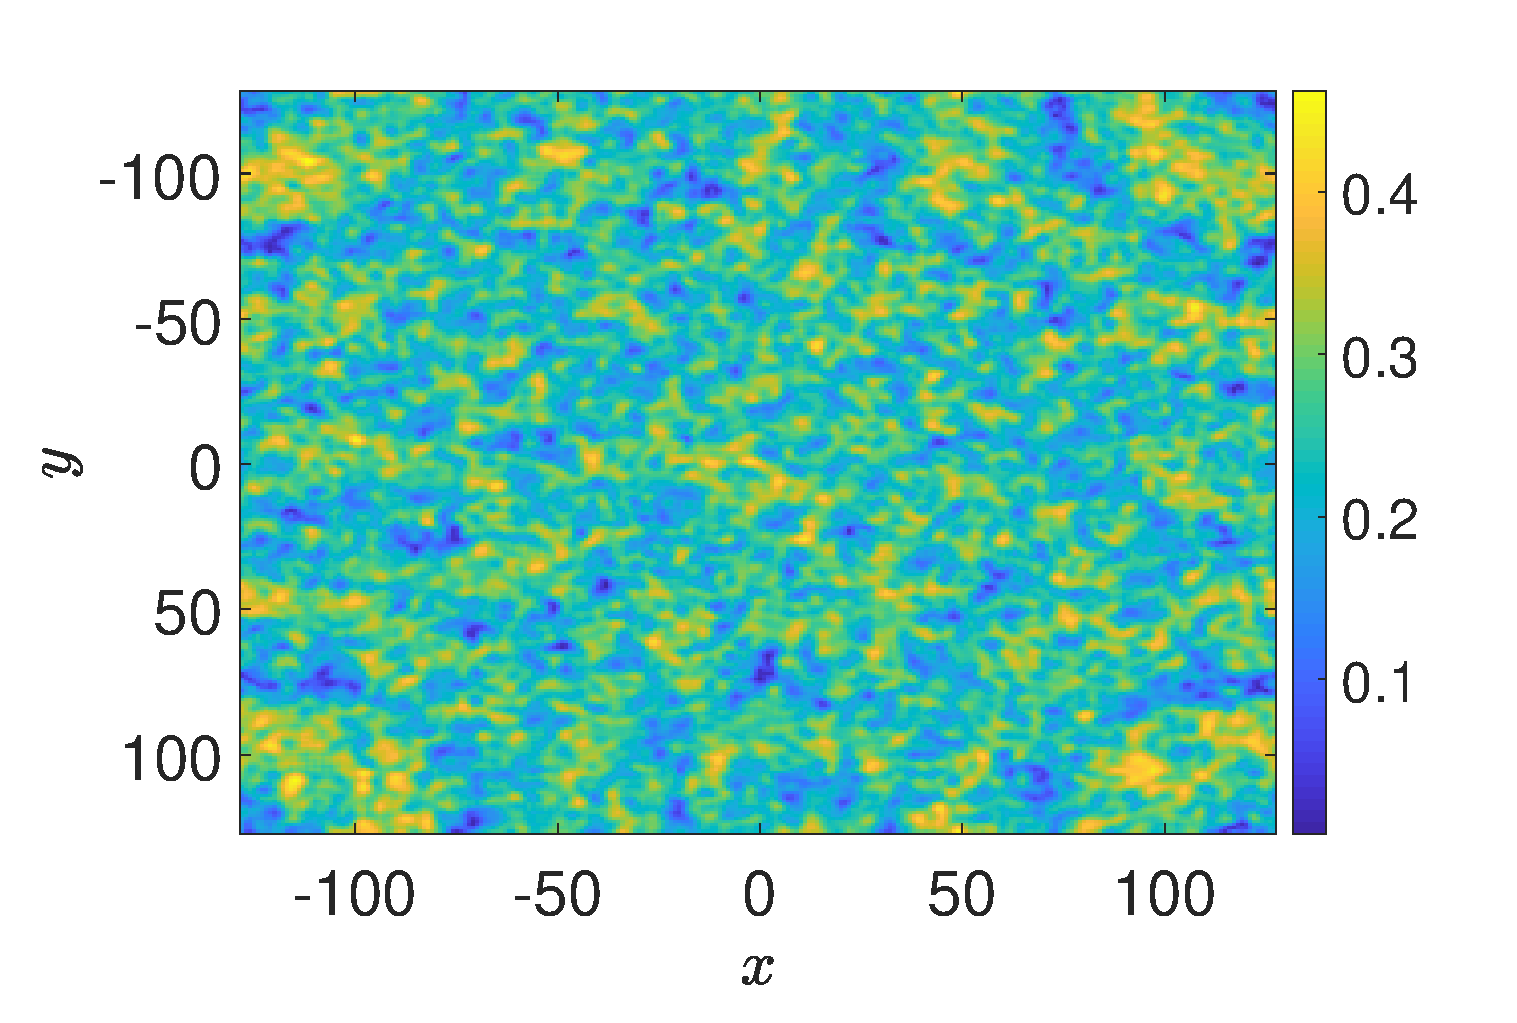
\includegraphics[width=.7\textwidth]{amplitude_K_128_Lx_128_tf_1pt5e4} \\
(a) \\
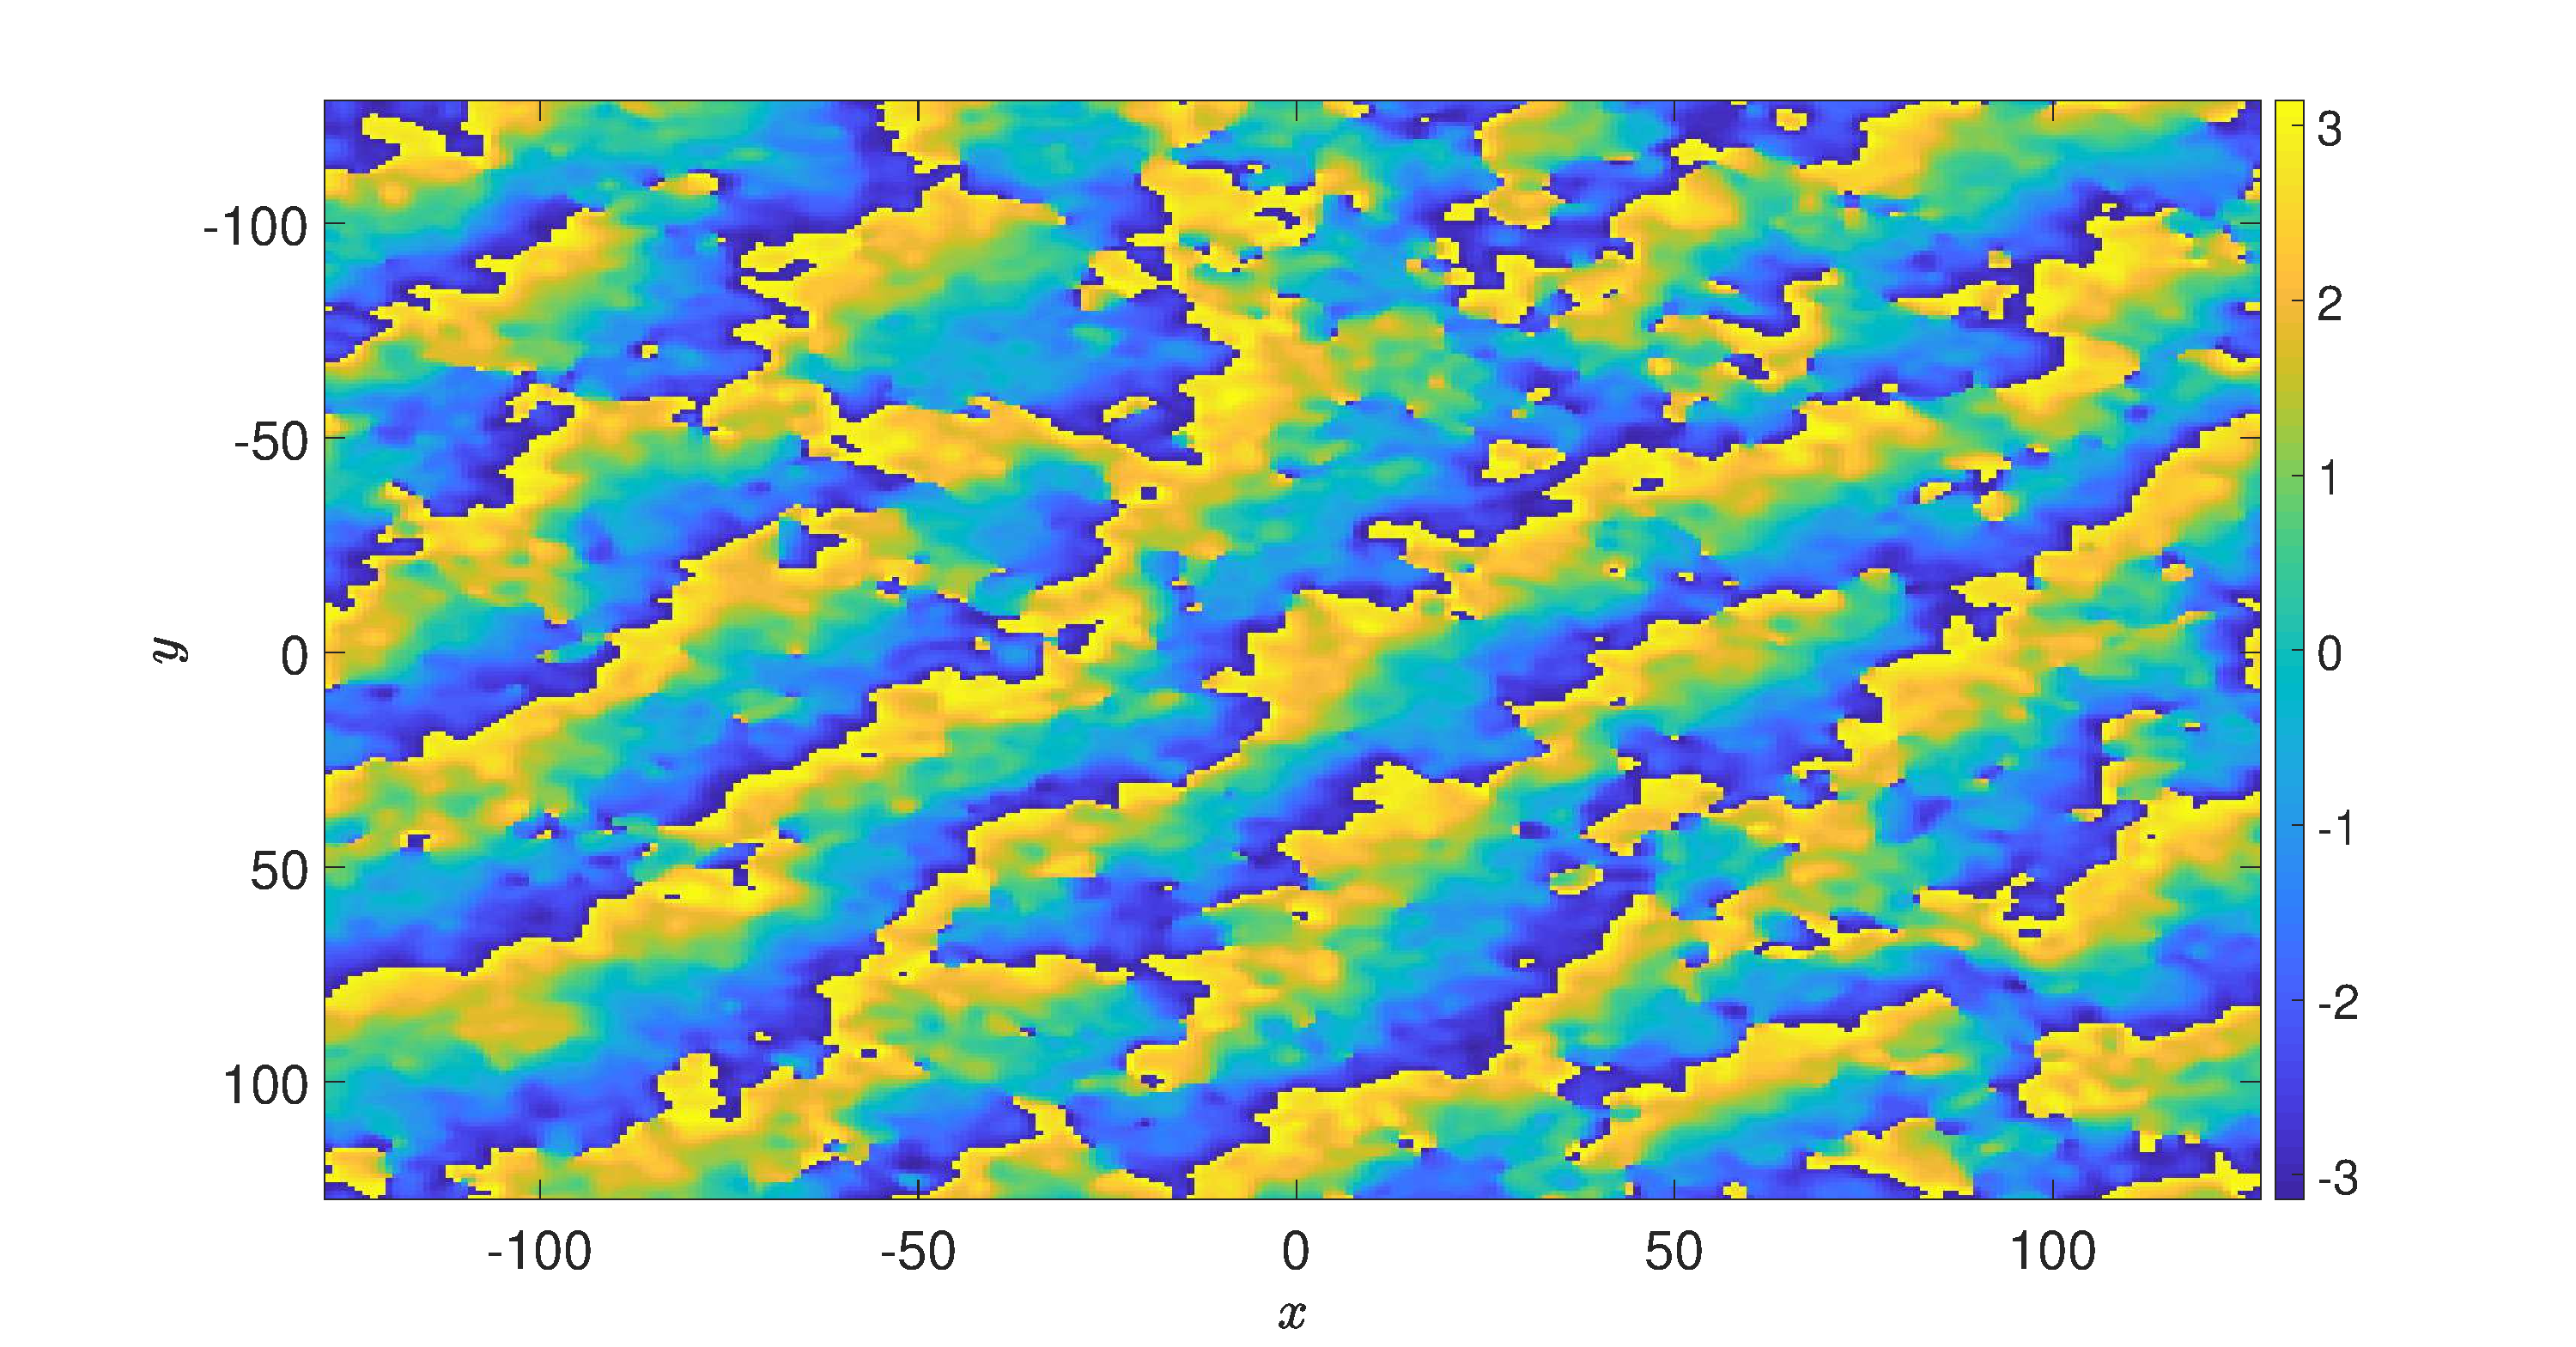
\includegraphics[width=.7\textwidth]{phase_K_128_Lx_128_tf_1pt5e4} \\
 (b) \\
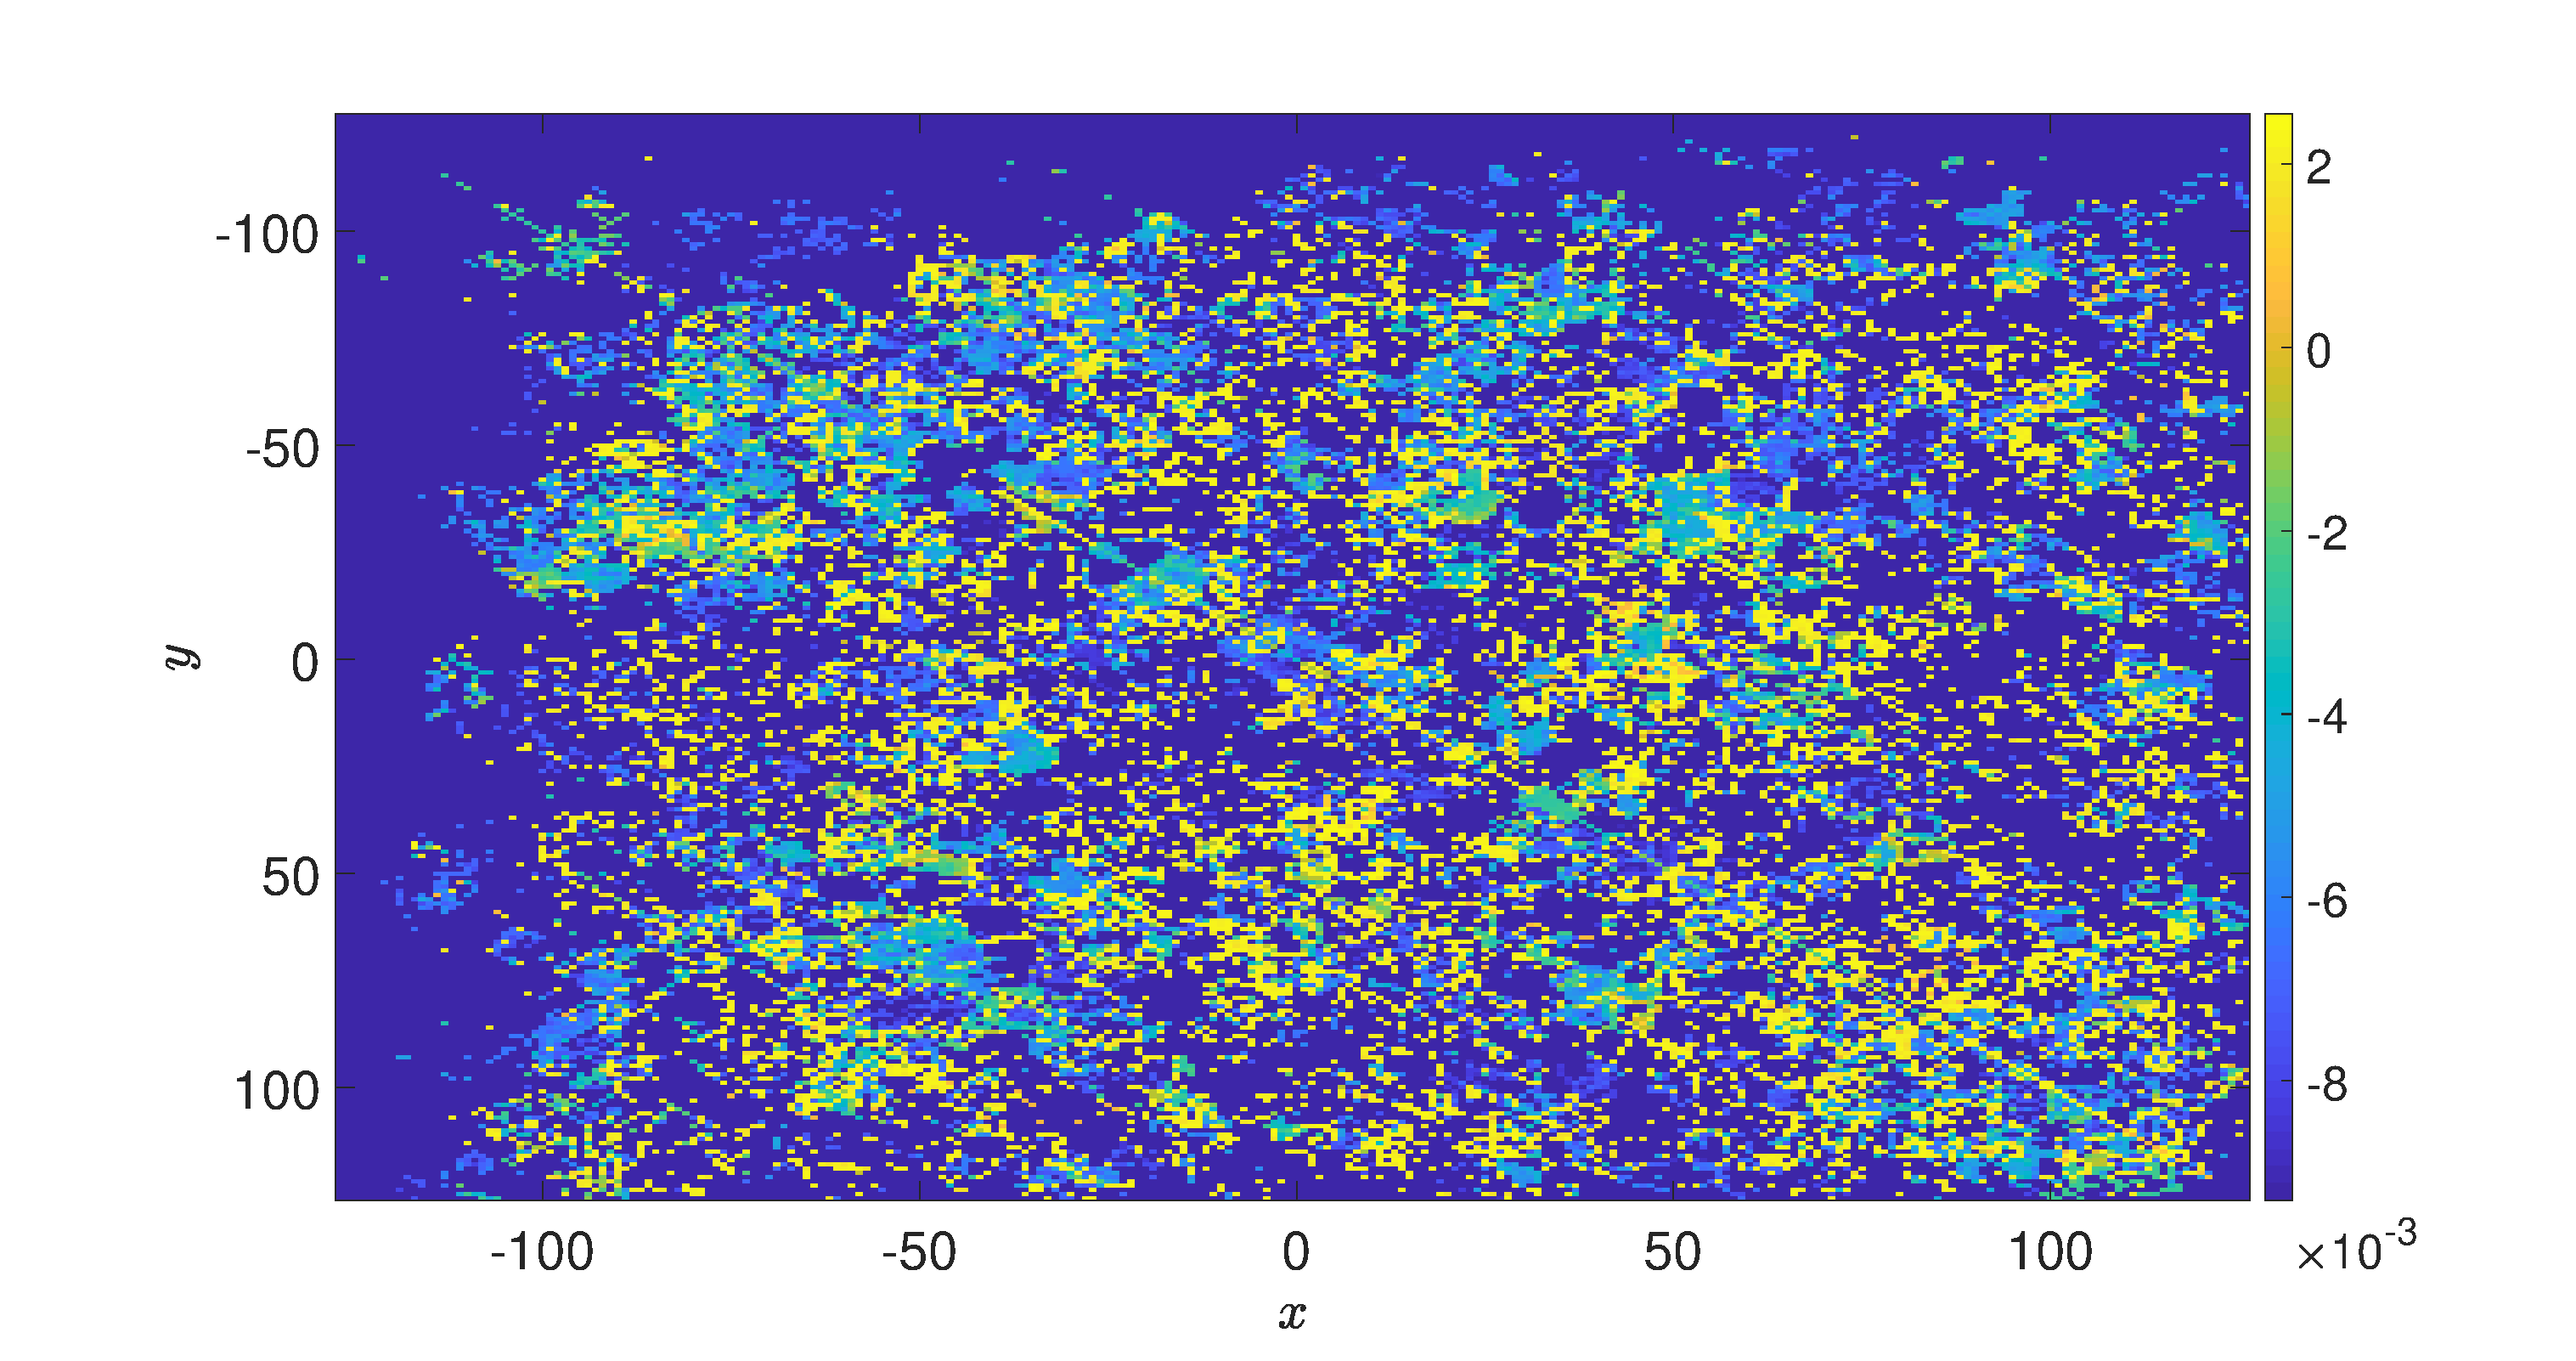
\includegraphics[width=.7\textwidth]{ftle_K_128_Lx_128_tf_1pt5e4} \\
(c)
\end{tabular}
\caption{The amplitude $\left|\psi(x,y,t_{f})\right|$ (a), phase $\mbox{arg}\left\{\psi(x,y,t_{f})\right\}$ (b), and FTLE field (c).  Note, while the flow is no longer strictly symmetric, the FTLE field still shows a strong remnant of it.}
\end{figure}

\begin{figure}[!h]
\centering
\begin{tabular}{c}
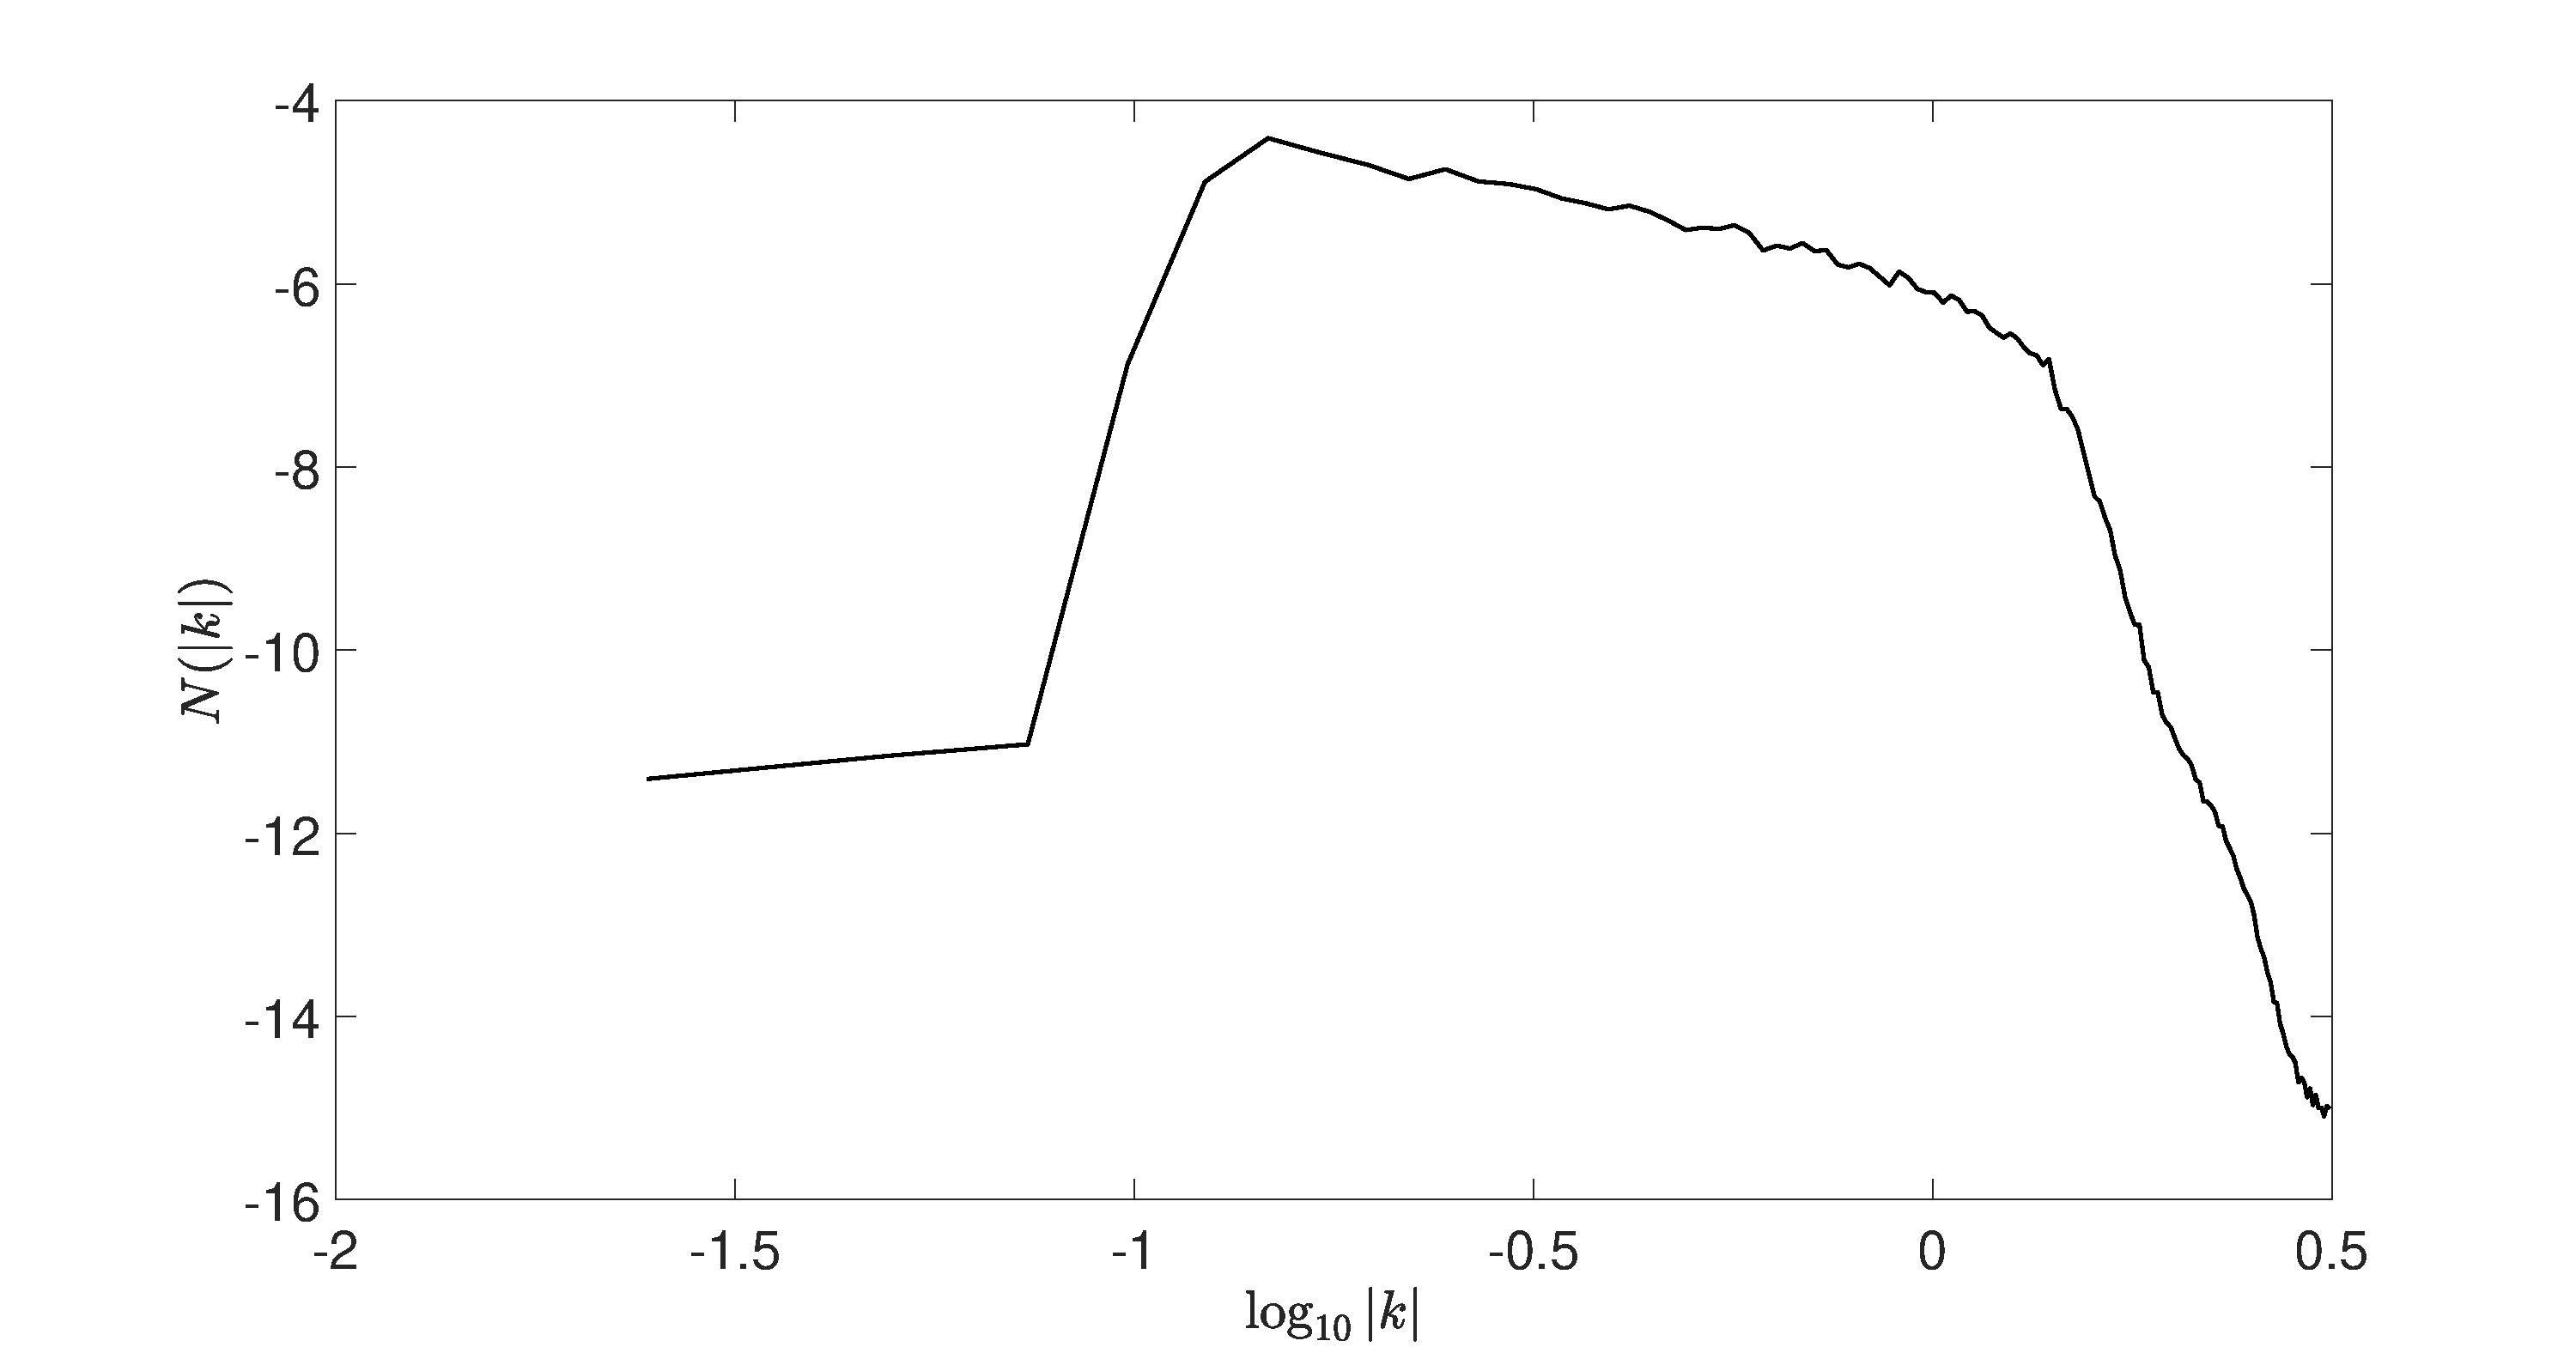
\includegraphics[width=.7\textwidth]{action_cascade_K_128_Lx_128_tf_1pt5e4} \\ 
(a) \\
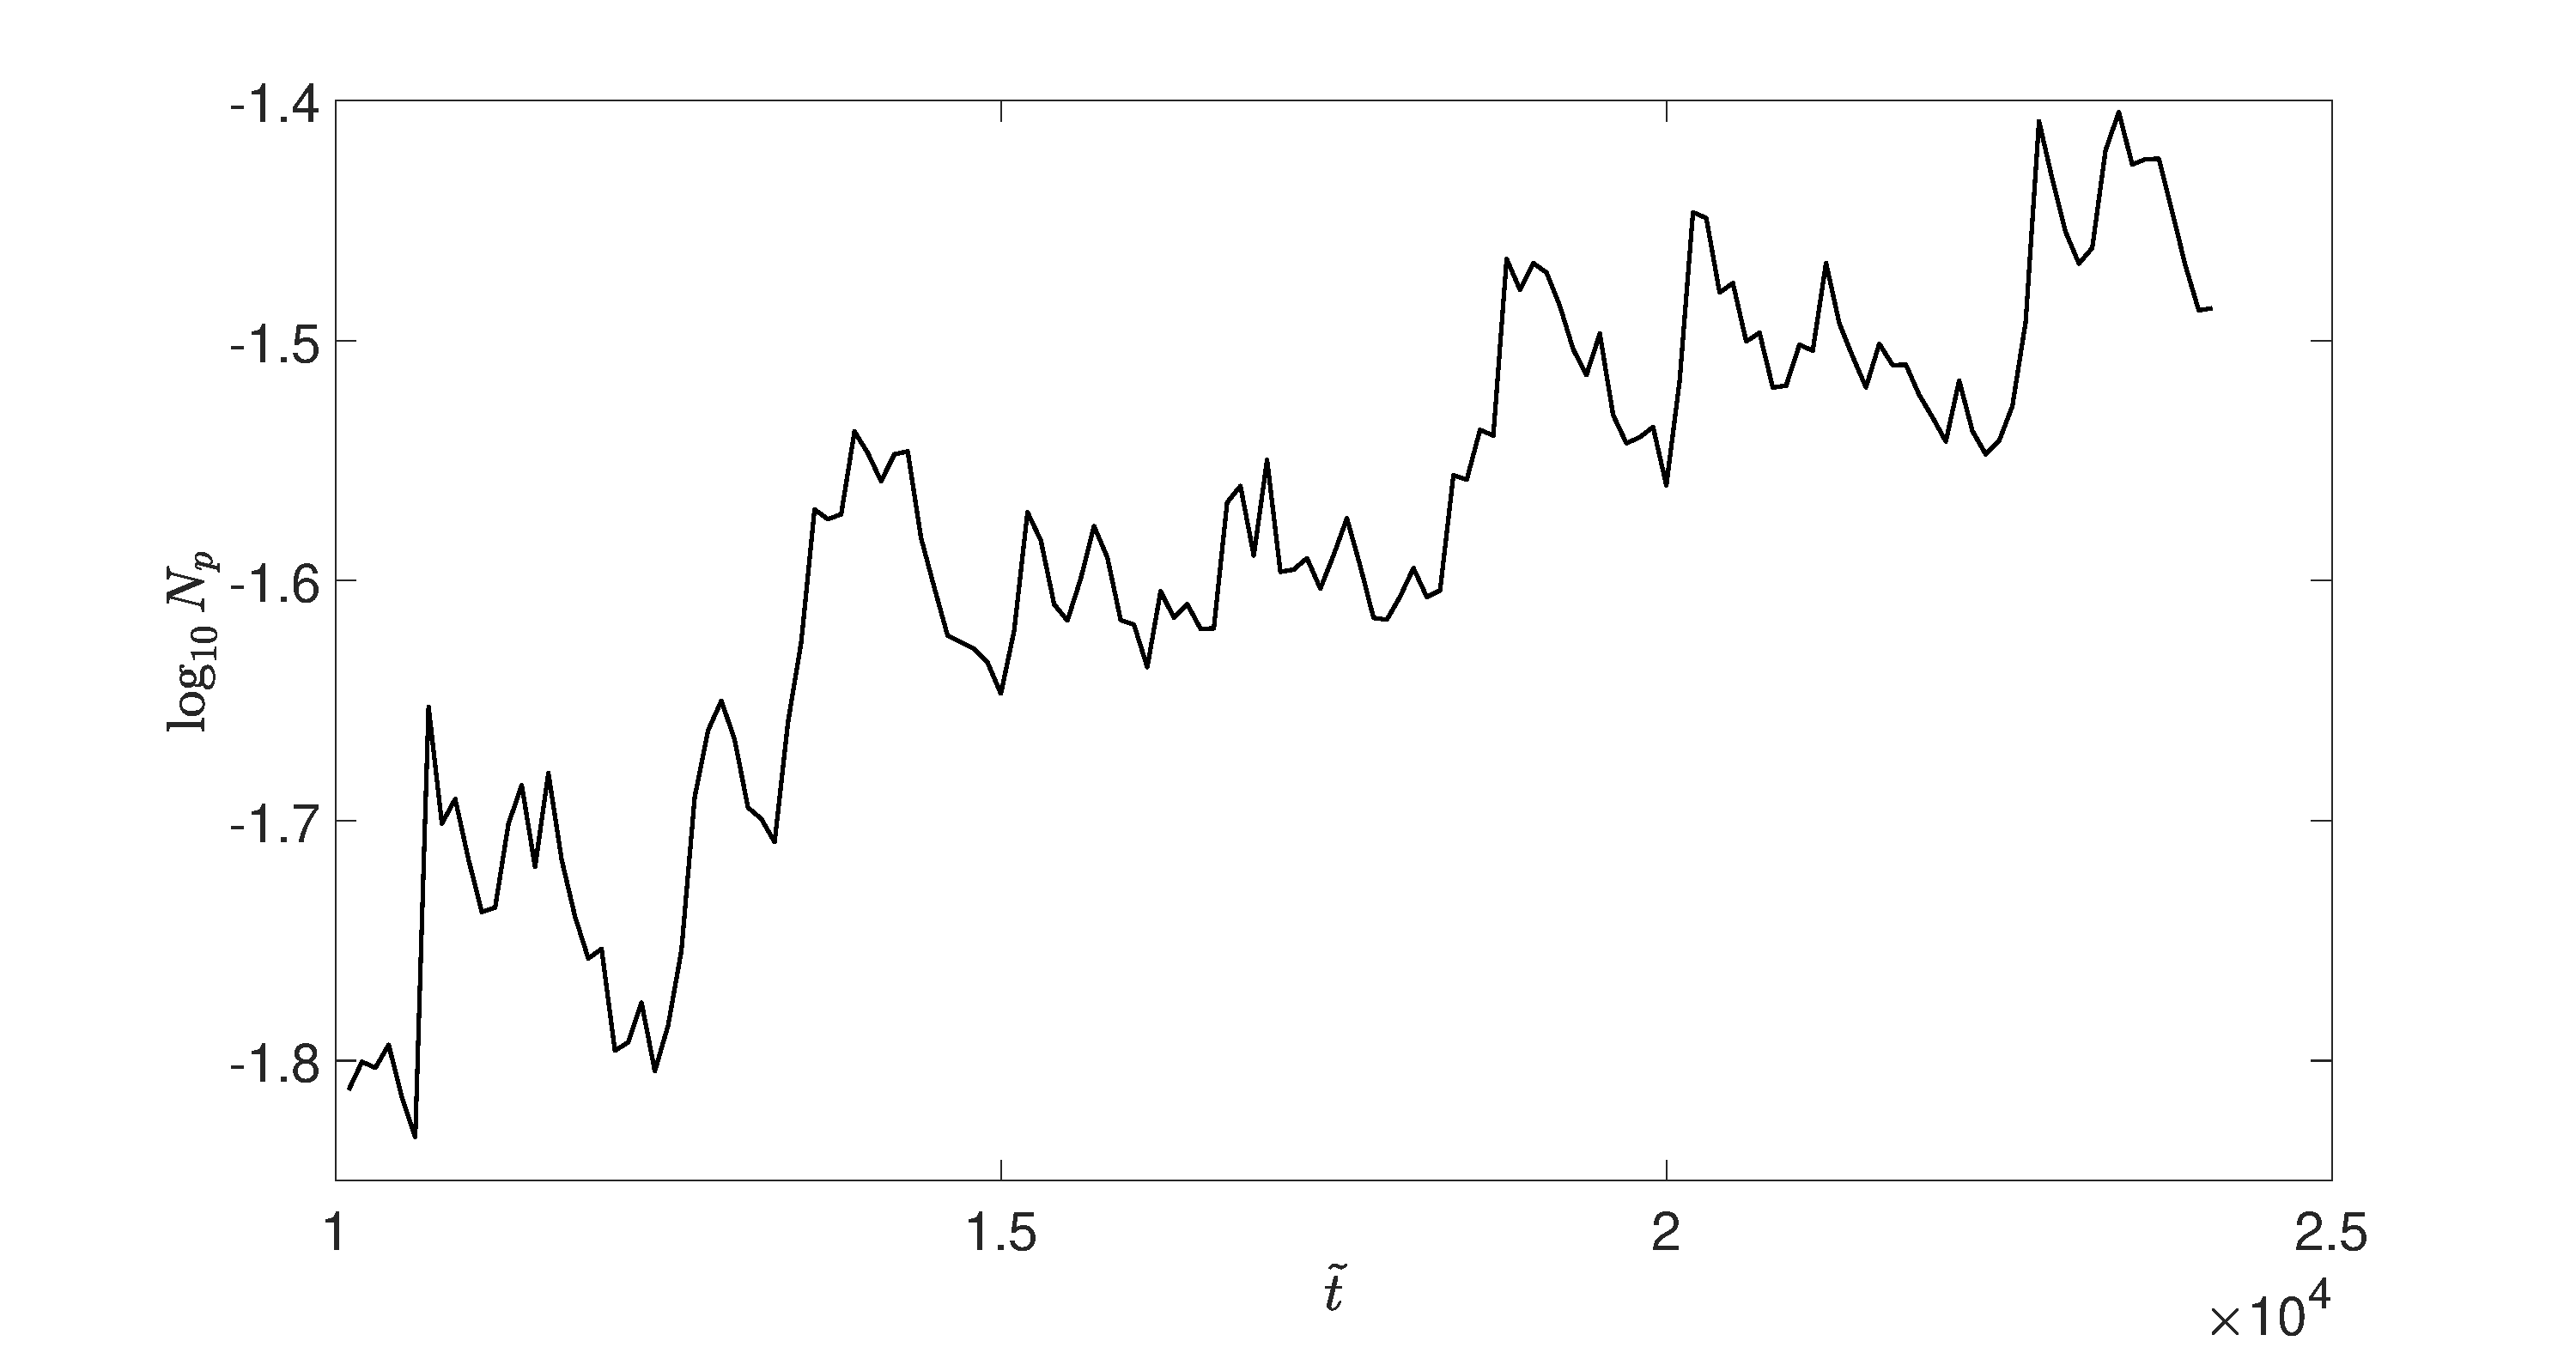
\includegraphics[width=.7\textwidth]{np_count_K_128_Lx_128_tf_1pt5e4}\\
(b)
\end{tabular}
\caption{The wave action $N(|k|)$ (a), and `particle count' $N_{p(t)}$ (b) .  An argument can be made that the plot of the particle count $N_{p}$ shows roughly when the system is in equilibrium. If you squint, and in some ways that's all Nazarenko and company do, you can see the right cascade rate in (a).}
\end{figure}

\begin{figure}
\centering
\begin{tabular}{c}
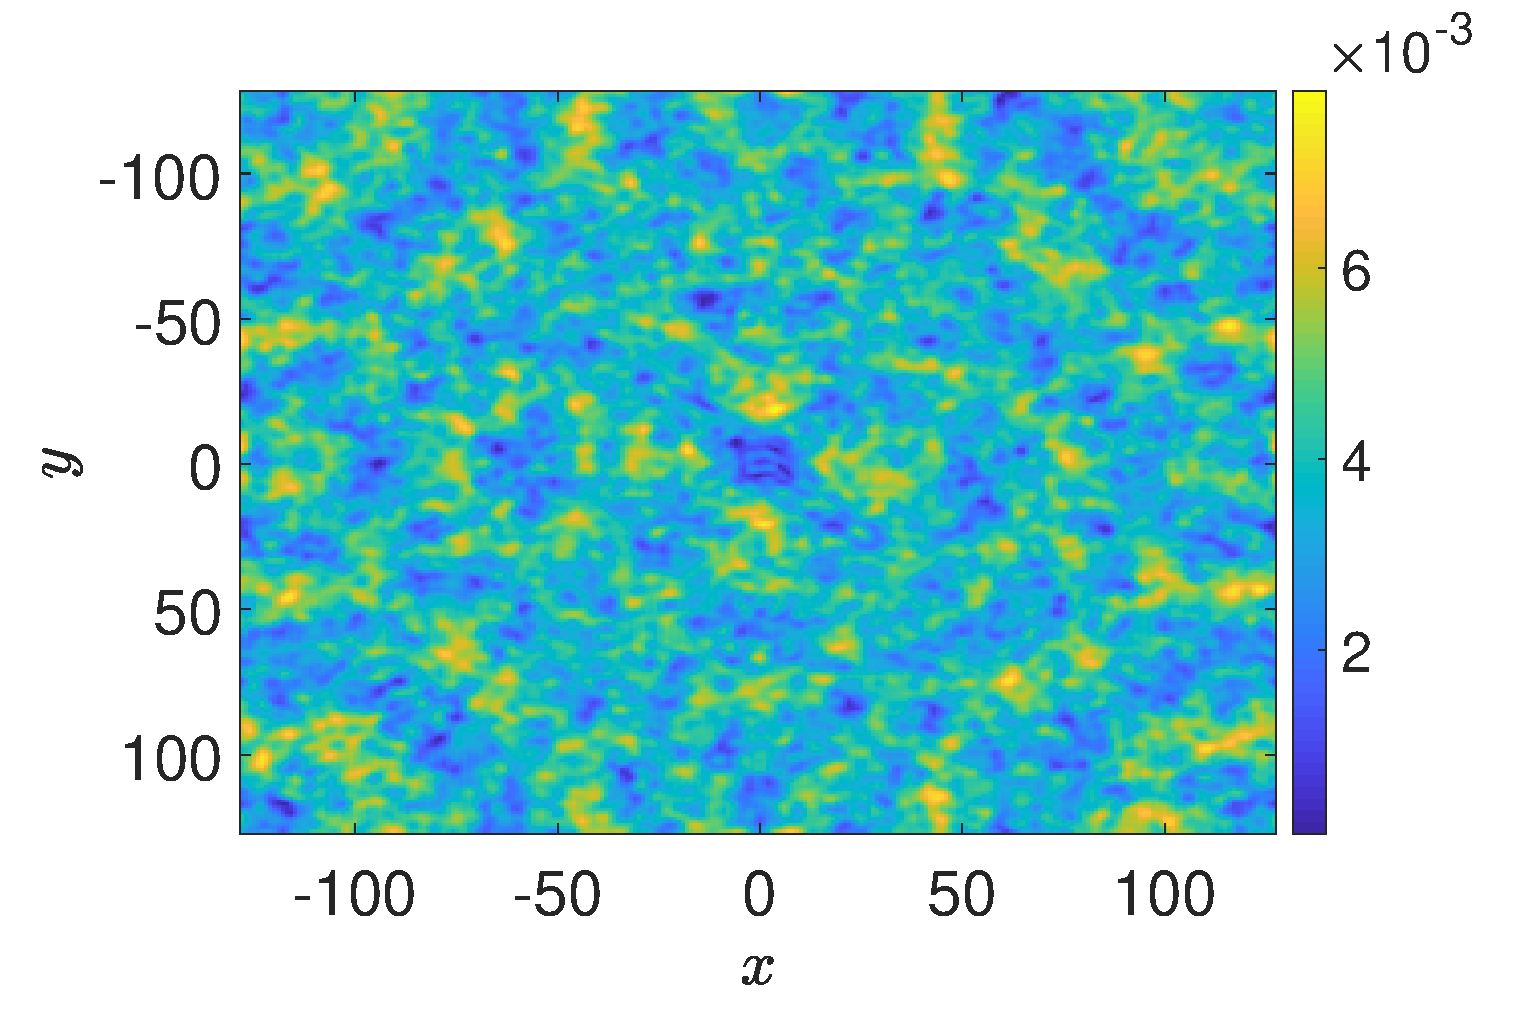
\includegraphics[width=.7\textwidth]{dmd_amplitude_K_128_Lx_128_tf_1pt5e4} \\
(a) \\
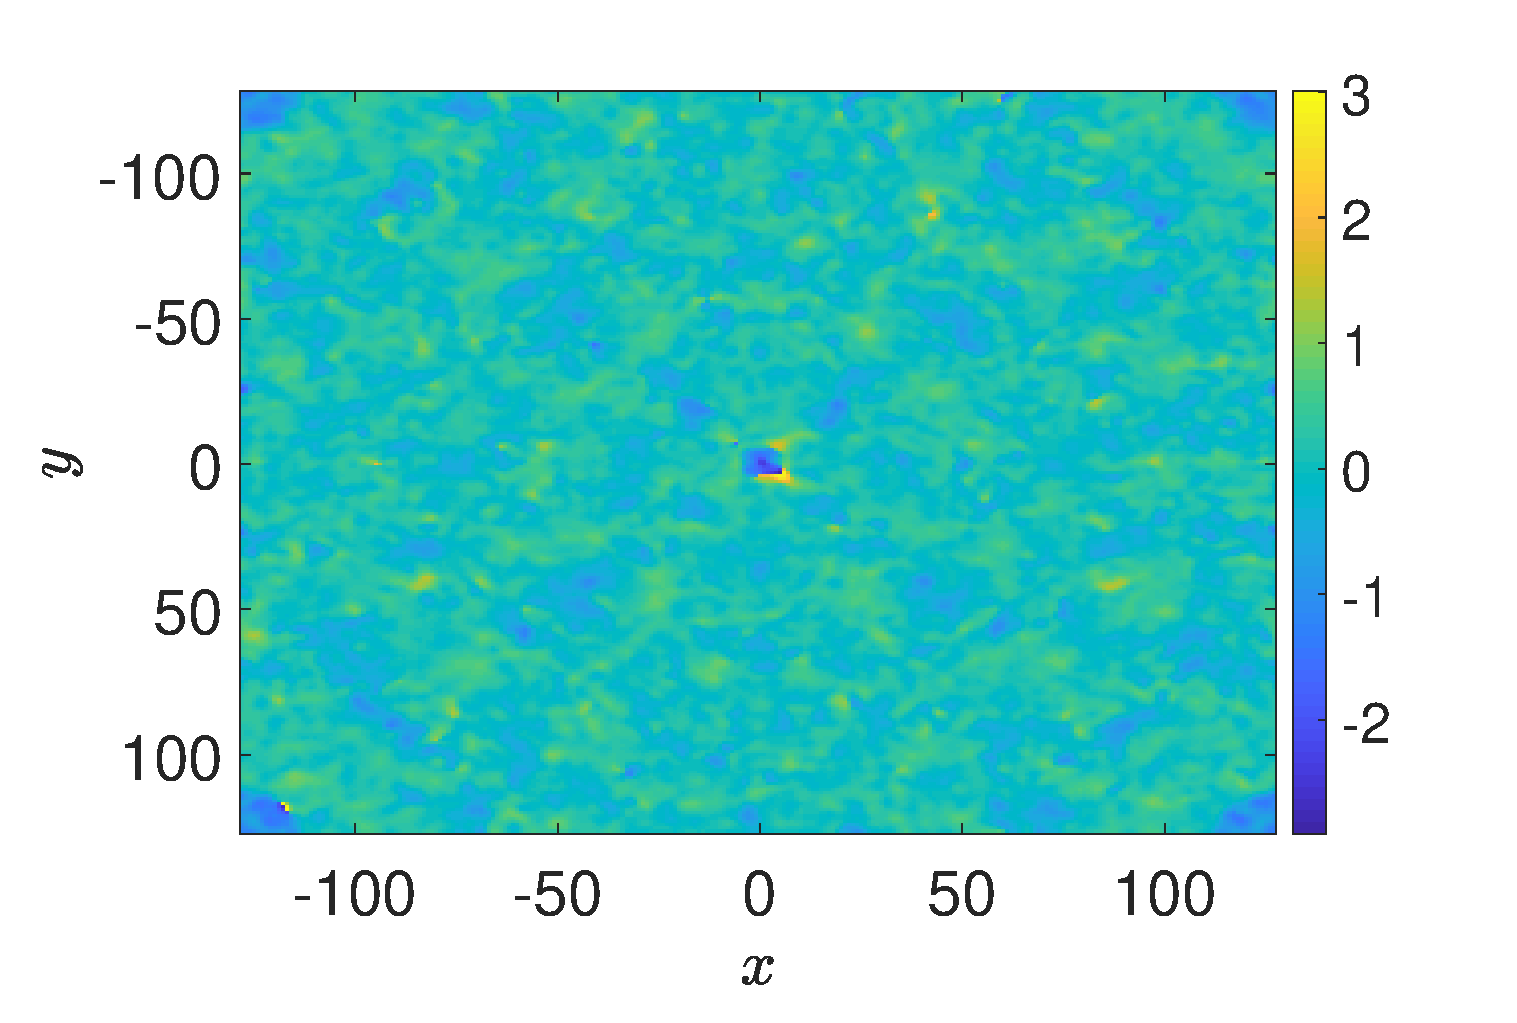
\includegraphics[width=.7\textwidth]{dmd_phase_K_128_Lx_128_tf_1pt5e4} \\
 (b) \\
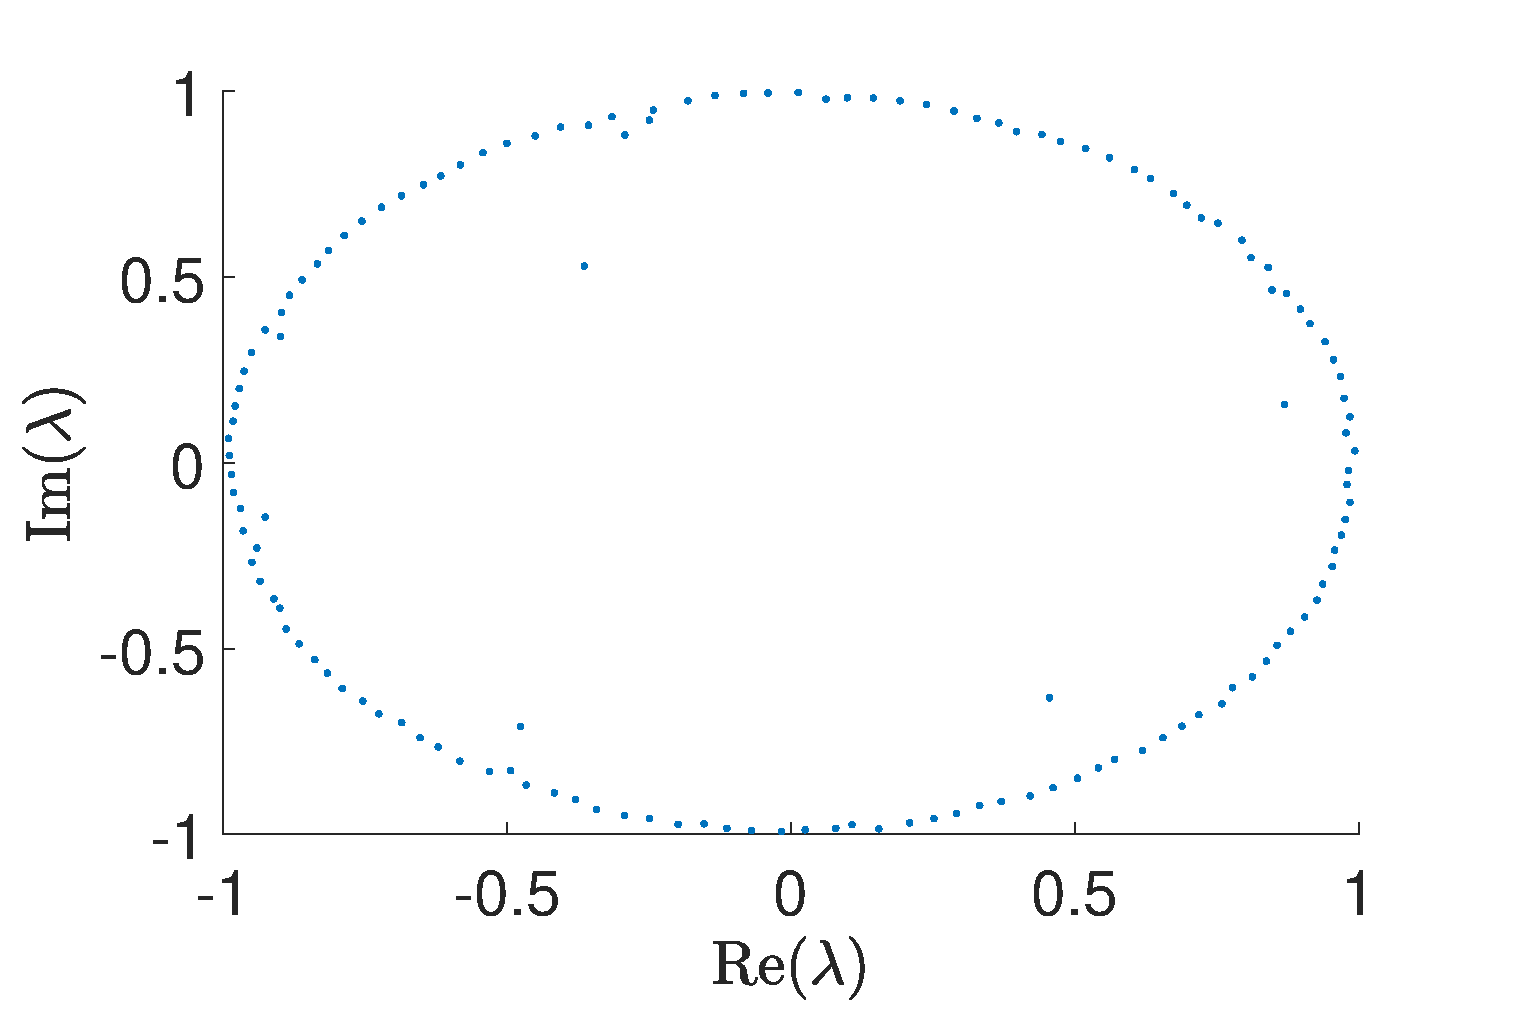
\includegraphics[width=.7\textwidth]{dmd_spectrum_K_128_Lx_128_tf_1pt5e4} \\
(c)
\end{tabular}
\caption{The amplitude (a) and phase (b) of the most unstable mode from the DMD, and the associated spectrum of the DMD (c).}
\end{figure}

\end{document}